\section{How the code was assembled}\label{sec:assembly}

The published text of the numerical-relativity particle-in-cell (NRPIC) method \cite{Wu:2026nrpic} provided the sole specification for the coupled Einstein-Vlasov solver built here without access to the original authors' code. This independent reconstruction tests whether the written equations and algorithmic rules fix the coupled method completely. The implementation assembles the coupled solver inside the host code AthenaK \cite{2026ApJS..283...27S,Zhu:2024utz} from existing capabilities across neighboring fields. AthenaK supplies the block-structured octree mesh with adaptive refinement, ghost-zone exchange, prolongation, and restriction. It also provides the Z4c spacetime solver in moving-puncture gauge, the particle container and drift update, the magnetohydrodynamics matter-source interface, and the pseudospectral apparent-horizon finder \cite{2026ApJS..283...27S,Zhu:2024utz}. Portable parallel execution of mesh stencils and particle loops comes from the Kokkos performance-portability library \cite{2022ITPDS..33..805T}.

Plasma particle-in-cell methods contribute implicit midpoint geodesic integration \cite{Bacchini:2020cze}, the velocity-space Boris rotation \cite{boris1970relativistic,1991ppcs.book.....B}, cloud-in-cell deposition with binomial filtering and compensation \cite{1988csup.book.....H,1991ppcs.book.....B}, and conservative single-level deposition across refinement boundaries \cite{Myers:2021gfn}. Numerical relativity and mesh methods supply the tetrad form of geodesic motion \cite{Olivares:2021cfa,Boyeneni:2025tsx}, lapse excision inside black holes \cite{Rosswog:2023nnl}, parabolic relaxation of the Hamiltonian constraint \cite{Duez:2002bn,Etienne:2024ncu}, and the L\"ohner refinement indicator \cite{1987CMAME..61..323L}. Exact analytical solutions for Kerr geodesics, Oppenheimer--Snyder dust collapse \cite{Oppenheimer:1939ue}, monoenergetic cluster equilibria \cite{1985ApJ...298...34S}, and homogeneous spheroid potentials complete the external inputs. This work combines those inputs into the two geodesic pushers in the symmetric and Cholesky tetrad gauges, cubic Hermite metric reconstruction, and single-level deposition with an optional level cap and compensated filtering. Additional components built here provide particle-coupled adaptive mesh refinement, lapse excision with interpolant-derivative apparent-horizon diagnostics, constraint-control terms, initial-data and validation suites, and the staggered coupled cycle.

Figure~\ref{fig:hypergraph} shows which capabilities each component combines. Horizontal rows list the existing capabilities grouped along the left margin by their origin. Vertical red columns represent the components built in this work as hyperedges of a hypergraph. Blue dots along each column mark the inherited capabilities joined by that hyperedge. Red rows at the bottom denote the geodesic-pusher and deposition components built here. Red dots on those bottom rows mark their reuse inside the adaptive-mesh and coupled-cycle hyperedges.

\begin{figure*}[t]
\centering
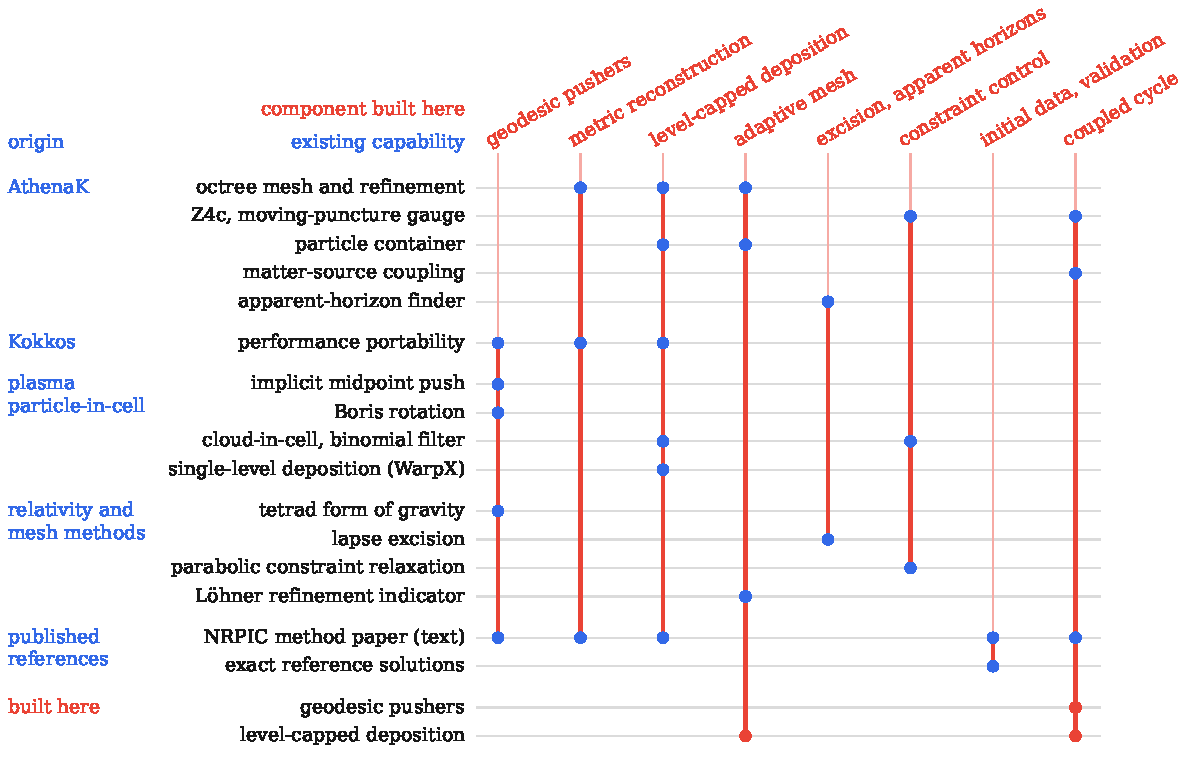
\includegraphics[width=\textwidth]{figures/fig_hypergraph.pdf}
\caption{The hypergraph shows how the code was assembled. Each row is a capability taken from an existing code or published method, grouped by origin. Each red column is a component built here, a hyperedge joining the capabilities it combines (dots). The red rows at the bottom are built components reused inside the coupled cycle and the adaptive mesh.}
\label{fig:hypergraph}
\end{figure*}

Large-language-model agents carried out the reconstruction under human direction across dedicated solver-development, verification, and manuscript roles. One model in the solver-development role wrote the derivations and solver source and directed the tests. Other models in the verification role built, ran, and analyzed the simulations, wrote independent reference solutions without access to the solver source, and audited the derivations, figures, and tables. A third model in the manuscript role wrote the text from the method specifications, figures, and test outcomes.

Candidate explanations for unexpected simulation results were tested against predictions recorded in advance. Each control run designed to test a stated explanation was preceded by a written prediction of the expected outcome. Seven initial explanations were refuted by these control runs. First, an apparent-horizon mass below $M$ after spherical collapse was attributed to early stopping of the pseudospectral flow finder. Calibration runs on an evolved vacuum black hole of known mass $M$ tested that explanation with a tighter stopping rule, which left the deficit unchanged. On the two finer meshes where the black hole is resolved, independent evaluations of the slice Misner--Sharp mass $M_{\rm MS}$ confirmed that the slice carried the mass $M$ (Fig.~\ref{fig:horizoncheck}; Table~\ref{tab:outcomes}). Direct inspection of the host code's finder showed that it interpolates a cell-centered metric-derivative array whose ghost zones retain their allocated zeros across mesh-block faces. Differentiation of the ghost-filled metric interpolant at those two cell sizes brought $M_{\rm AH}$ into agreement with $M_{\rm MS}$ on saved slices and in a live run. In Sec.~\ref{sec:dust}, three further initial explanations failed predictive controls: collapse dynamics for post-excision mass drift, harmlessness of one-level cloud coarsening, and the lattice beat alone for coarser-cloud disturbances. In Sec.~\ref{sec:clusters}, three more failed: sampling noise for the plain-filter bounce, sampling noise for the core oscillation, and second-order cell-size error for that oscillation. Independent audits of initial-data code and appendix tables against saved outputs caught two derivation slips and exposed unsupported log entries that were then corrected. In particular, redeposition from stored particles showed that a central-density excess under coarser clouds, first logged as matching the cycloid, came from the particle lattice beating against virtual cloud cells. Every effect without an isolating run has its cause stated in Sec.~\ref{sec:selfgravity} as not determined.

All materials needed to inspect and extend the simulations are public alongside the solver source code. The public release includes the simulation inputs, the analysis scripts, and the chronological record of every prediction and outcome. Readers can rerun the validation benchmarks, modify individual stages of the particle-mesh cycle, or audit each diagnostic test from those materials. The data-and-code-availability statement before the appendices gives the archive location.
